\documentclass{beamer}
\usetheme{default}
\beamertemplatenavigationsymbolsempty
\usepackage{rembeamer}

\begin{document}

\begin{frame}
  \begin{itemize}
    \item[] 
      Using the normal distribution to construct confidence intervals
      for a difference in proportions, and interpreting the results.
  \end{itemize}
\end{frame}

\begin{frame}
  \frametitle{An Psychology Example}
  \begin{itemize}
    \item[] 
      Question: do you want to buy a DVD for a discounted price of
      \$15? 
      \vspace{0.5cm}
    \item[] 
      \begin{smallitemize}
        \item
          Buy the DVD.
        \item
          Don't buy the DVD.
      \end{smallitemize}
      \vspace{0.5cm}
    \item[] 
      \begin{smallitemize}
        \item
          Buy the DVD.
        \item
          Don't buy the DVD, and keep the \$15 for other purchases.
      \end{smallitemize}
      \vspace{0.5cm}
    \item[] 
      150 subjects, 75 in each group. 
  \end{itemize}
\end{frame}

\begin{frame}
  \frametitle{Contingency Table}
  \begin{table}
    \begin{tabular}{@{}cccc@{}}
      \toprule
      Group & Buy & Do Not Buy & Total \\
      \cmidrule(r){1-1} \cmidrule(rl){2-2} \cmidrule(rl){3-3}
      \cmidrule(l){4-4}
      Control & 56 & 19 & 75 \\[0.3em]
      Treatment & 41 & 34 & 75 \\[0.3em]
      Total & 97 & 53 & 150 \\
      \bottomrule
    \end{tabular}
  \end{table}
\end{frame}

\begin{frame}
  \frametitle{Statistics and Hypotheses}
  \begin{displaymath}
    \begin{array}{rcl}
      \hat{p}_T - \hat{p}_C & = & \frac{34}{75} - \frac{19}{75} =
      0.453 - 0.253 = 0.200 \\[0.5cm]
      p_T - p_C & = & ? \\[0.5cm]
      p_T - p_C & \in & [0.190, 0.210]? \\[0.5cm]
      _T - p_C & \in & [0.199, 0.201]? \\[0.5cm]
      p_T - p_C & \in & [0.150, 0.250]? \\[0.5cm]
      p_T - p_C & \in & [0, 0.4]?
    \end{array}
  \end{displaymath}
\end{frame}

\begin{frame}
  \frametitle{Normal Distribution}
  \centering
  \begin{tikzpicture}
    \begin{axis}[
        ytick=\empty,
      ]
      \addplot [
        domain=-3:3,
        samples=200,
      ]
      {exp(-x^2 / (2)) / (sqrt(2*pi))};
    \end{axis}
  \end{tikzpicture}
\end{frame}

\begin{frame}
  \frametitle{Normal Distribution}
  \centering
  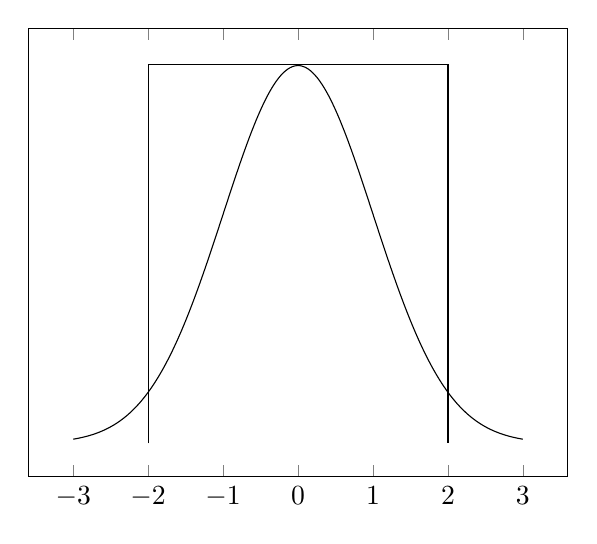
\begin{tikzpicture}
    \begin{axis}[
        ytick=\empty,
      ]
      \addplot [
        domain=-3:3,
        samples=200,
      ]
      {exp(-x^2 / (2)) / (sqrt(2*pi))};
      \draw (-2,0) -- (-2,0.4) -- (2,0.4) -- (2,0);
    \end{axis}
  \end{tikzpicture}
  \begin{equation*}
    95\% \implies [-1.96, 1.96]
  \end{equation*}
\end{frame}

\begin{frame}
  \frametitle{Calculating Confidence Intervals}
  \begin{displaymath}
    \begin{array}{rcl}
      95\% & \implies & [-1.96, 1.96] \\[1em]
      \mu & = & \text{mean} \\[1em]
      \sigma & = & \text{standard deviation} \\[1em]
      95\%& = & [\mu - (1.96) \sigma, \mu +
      (1.96) \sigma] \\[1em]
      \mu & = & 0.200 \\[1em]
      \sigma & = & \text{SE} = 0.076 \\[1em]
      95 & = & [0.200 - (1.96)(0.076), 0.200 + (1.96)(0.076)] \\[1em]
      & = & [0.051, 0.349]
    \end{array}
  \end{displaymath} 
\end{frame}

\begin{frame}
  \frametitle{Normal Distribution}
  \centering
  \begin{tikzpicture}
    \begin{axis}[
        ytick=\empty,
      ]
      \addplot [
        domain=0:0.4,
        samples=200,
      ]
      {exp(-(x-0.2)^2 / (2*((0.076)^2))) / (sqrt(2*pi*((0.076)^2)))};
      \draw (0.051,0) -- (0.051,5.25) -- (0.349,5.25) -- (0.349,0);
    \end{axis}
  \end{tikzpicture}
  \begin{equation*}
    95\% \implies [0.051. 0.349]
  \end{equation*}
\end{frame}

\end{document}

